\documentclass[100,a4paperpaper,]{article}

  \title{\textbf{\textcolor{white}{Relatório de Conjuntura}}}
  \author{\textbf{\textcolor{white}{Política Fiscal}}}
  \date{\textbf{\textcolor{white}{\today}}}
  


\newcommand{\logo}{logo-banestes-transparente.png}
\newcommand{\cover}{cover-banestes-menor.png}
\newcommand{\logotitle}{logo-banestes-branca.png}
\newcommand{\iblue}{004b8d}
\newcommand{\igray}{d4dbde}
\usepackage{booktabs}
\usepackage{longtable}
\usepackage{array}
\usepackage{multirow}
\usepackage{wrapfig}
\usepackage{float}
\usepackage{colortbl}
\usepackage{pdflscape}
\usepackage{tabu}
\usepackage{threeparttable}
\usepackage{threeparttablex}
\usepackage[normalem]{ulem}
\usepackage{makecell}
\usepackage{xcolor}

% Author: Karol KozioL
% License: GPL-3
% Modified by: Sarah Wagner

% % % packages -----------------------------------------------------------------------------------
\usepackage{amsmath}
\usepackage{array}
\usepackage{booktabs}
\usepackage{calc}
\usepackage{eso-pic}
\usepackage[left = 30pt, right = 30pt, top = 25pt, bottom = 25pt, headsep = 40pt, includeheadfoot]{geometry}
\usepackage{fancyhdr}
\usepackage{fontspec}
\usepackage{graphicx}
\usepackage[utf8]{inputenc}
\usepackage{lastpage}
\usepackage{multirow}
\usepackage{tabularx} 
\usepackage{tikz}
\usepackage{titlesec}
\usepackage{titling}
\usepackage{xcolor, colortbl}
\usepackage{etoolbox}
\usepackage{ragged2e}
\usepackage{xcolor}
\usepackage[fontsize=14]{scrextend}
\usepackage[portuguese]{babel}
\usepackage{indentfirst}

% % % settings -----------------------------------------------------------------------------------

% % custom colors
\definecolor{iblue}{HTML}{\iblue}
\definecolor{igray}{HTML}{\igray}

% definition of pagename
\newcommand\pagename{Page}

% % fonts 
\defaultfontfeatures{Mapping = tex-text}
\setmainfont{Arial}
\newfontfamily\headingfont{Arial}



% % sections
\titleformat{\section}{\color{iblue}\headingfont\Large\bfseries}{\thesection}{1em}{}[\titlerule]
\titleformat{\subsection}{\color{iblue}\headingfont\large\bfseries}{\thesubsection}{1em}{}
\titleformat{\subsubsection}{\color{iblue}\headingfont\large\bfseries}{\thesubsubsection}{1em}{}

% % misc
\setlength{\parindent}{0em} 
\setlength{\parskip}{1em}
\linespread{1.15}
\renewcommand{\baselinestretch}{1.25}
\raggedright
\newcolumntype{C}{>{\centering\arraybackslash}X}
\justifying


% % % custom titlepage ----------------------------------------------------------------------------
\newcommand\BackgroundPic{%
	\put(0,0){%
		\parbox[b][\paperheight]{\paperwidth}{%
			\vfill
			\centering
			
\includegraphics[width=\paperwidth,height=\paperheight]{\cover}%
			\vfill
}}}

\makeatletter

% pagestyle titlepage
\fancypagestyle{customtitle}{
	\lhead{}
	\chead{}
	\rhead{\includegraphics{\logotitle}}
	\makeatother
	\lfoot{}
	\cfoot{}
	\rfoot{}
}


% titlepage
\renewcommand{\maketitle}{
	\thispagestyle{customtitle}
	\AddToShipoutPicture*{\BackgroundPic}
	\ClearShipoutPicture
	
	\phantom{a}\hfill
	\vspace{12cm}
	
	\begin{tabular}[l]{@{}p{\textwidth}@{}}
		\color{iblue}\headingfont\LARGE\@title\\[1em]
		\color{iblue}\headingfont\Large\@author\\[1em]
		\color{iblue}\headingfont\large\@date\\[1em]
	\end{tabular}
	
	
	\clearpage
}

\makeatother

% % % header and footer ---------------------------------------------------------------------------
\pagestyle{fancy}
\lhead{}
\chead{}
\rhead{ 
\includegraphics{\logo}}
\makeatother
\newlength{\myheight}
\lfoot{}
\cfoot{}
\rfoot{\pagename~\thepage \hspace{1pt} / \pageref{LastPage}}
\renewcommand\headrulewidth{0pt}
\renewcommand\footrulewidth{0pt}




\begin{document}


\renewcommand{\contentsname}{Sumário}


\maketitle
\tableofcontents
\clearpage

\section{Estatísticas Fiscais: Análise acima da linha} 
 \vspace{0.5cm}

Passado o pior momento da pandemia, que exigiu uma série de gastos
extraordinários e não previstos no orçamento fiscal, as contas públicas
começaram a se ajustar em 2021.

Em setembro, o resultado primário do Governo
Central\footnote{O Governo Central é composto por Banco Central, Tesouro Nacional e Previdência Socal.},
calculado à partir da diferença entre receitas e despesas, gerou um
superávit de R\$ 302 milhões a preços correntes. Este resultado registra
um aumento significativo em comparação ao mesmo período do ano passado,
no qual o Governo Central obteve déficit de R\$ 76,1 bilhões.

O quadro explica-se principalmente pela elevação das receitas (aumento
de 20 \%), em especial o aumento de 34\% nas receitas administradas pela
Receita Federal. Ao passo que houve redução de 30\% nas despesas,
motivado principalmente pela queda nos gastos necessários para reduzir o
impacto da pandemia no país. Em comparação com setembro do ano passado,
as despesas do Governo Central relacionadas ao combate ao COVID-19
reduziram-se cerca de 82\%.

Além disso, em relação ao acumulado de janeiro a setembro, o Governo
Central obteve déficit de R\$ 82,4 bilhões. Em termos reais, este
resultado destaca uma redução no déficit em aproximadamente de 88\%, em
comparação ao mesmo período do ano passado.

\begingroup\fontsize{13}{15}\selectfont

\begin{longtable}[t]{lrrrr}
\caption{\label{tab:Tabela Gov Central}Resultado do Governo Central}\\
\toprule
\multicolumn{1}{c}{} & \multicolumn{2}{c}{SETEMBRO} & \multicolumn{2}{c}{ACUMULADO DO ANO} \\
\cmidrule(l{3pt}r{3pt}){2-3} \cmidrule(l{3pt}r{3pt}){4-5}
Discriminação & 2020 & 2021 & 2020 & 2021\\
\midrule
\endfirsthead
\caption[]{Resultado do Governo Central \textit{(continued)}}\\
\toprule
\multicolumn{1}{c}{} & \multicolumn{2}{c}{SETEMBRO} & \multicolumn{2}{c}{ACUMULADO DO ANO} \\
\cmidrule(l{3pt}r{3pt}){2-3} \cmidrule(l{3pt}r{3pt}){4-5}
Discriminação & 2020 & 2021 & 2020 & 2021\\
\midrule
\endhead

\endfoot
\bottomrule
\multicolumn{5}{l}{\rule{0pt}{1em}\textit{Fonte:} Tesouro Nacional}\\
\endlastfoot
Receital Total (1) & 121.996 & 151.804 & 1.012.942 & 1.370.199\\
Transf. por Repartição de Receita (2) & 15.374 & 23.356 & 187.039 & 252.228\\
Receita Líquida (1 - 2) & 106.621 & 128.448 & 825.903 & 1.117.971\\
Despesa Total (3) & 182.766 & 128.146 & 1.503.350 & 1.200.457\\
Resultado Primário Governo Central (3 - 4) & -76.144 & 303 & -677.446 & -82.486\\*
\end{longtable}
\endgroup{}

\newpage

\section{Estatísticas Fiscais: Análise abaixo da linha} 
 \vspace{0.5cm}

Para a análise do resultado primário do setor público consolidado --
composto pelo Governo Federal, estados, municípios e empresas estatais,
exceto Petrobrás e Eletrobrás -- é utilizado o conceito de Necessidade
de Financiamento do Setor Público (NFSP). A NFSP refere-se a variação do
saldo da dívida pública, portanto, variações positivas significam
déficit, enquanto variações negativas correspondem a superávit.

Em setembro, o setor público consolidado obteve superávit primário de
R\$ 12,9 bilhões, resultado positivo em comparação ao déficit de R\$
64,5 bilhões registrado em setembro do ano passado. No acumulado do ano,
o superávit primário foi de R\$ 14,1 bilhões, em relação ao ano passado,
houve melhora no resultado fiscal, visto que o período fechou com
déficit de R\$ 635 bilhões (11\% do PIB).

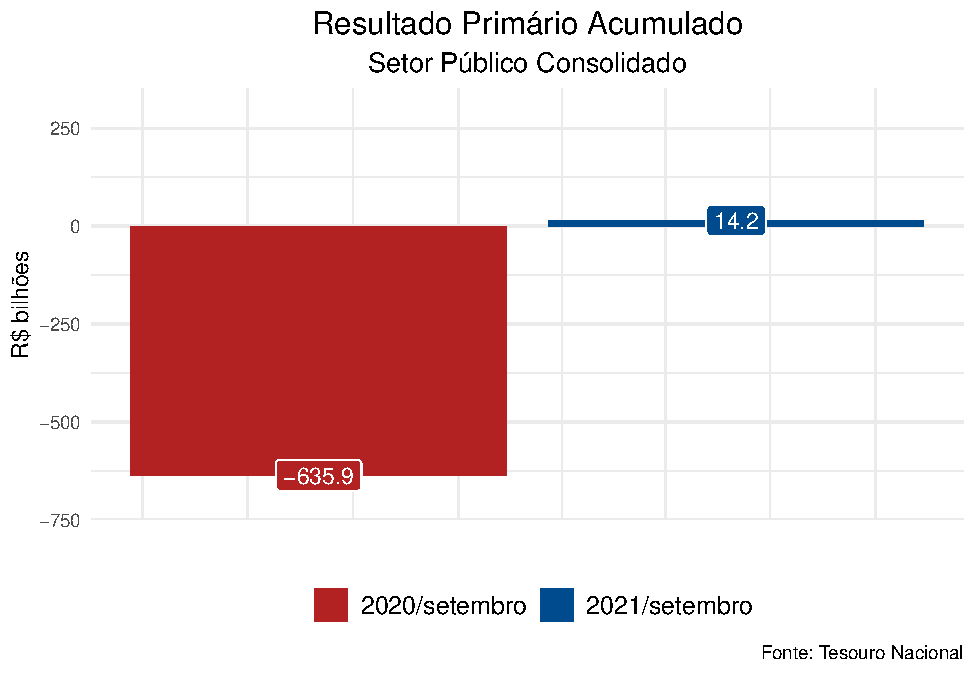
\includegraphics{politica-fiscal_files/figure-latex/setor publico consolidado-1.pdf}

A dívida líquida do setor público (DLSP), que inclui os passivos do
governo exceto o pagamento de juros, fechou o mês de setembro no patamar
de R\$ 4,8 trilhões, cerca de 58,5\% do PIB. Redução de 0,9 pontos
percentuais em relação ao mês anterior e aumento de 10,4\% comparado a
setembro de 2020.

No que se refere a dívida bruta do governo geral (DBGG), verifica-se uma
trajetória ascendente em relação ao PIB desde 2015. É importante
salientar que a relação dívida/PIB é um dos principais indicares fiscais
quanto a sustentabilidade da dívida. Em setembro deste ano, o saldo da
DBGG foi de R\$ 6,9 trilhões, o que corresponde a 83\% do PIB, aumento
de 0,3 pontos percentuais comparado a agosto deste ano.

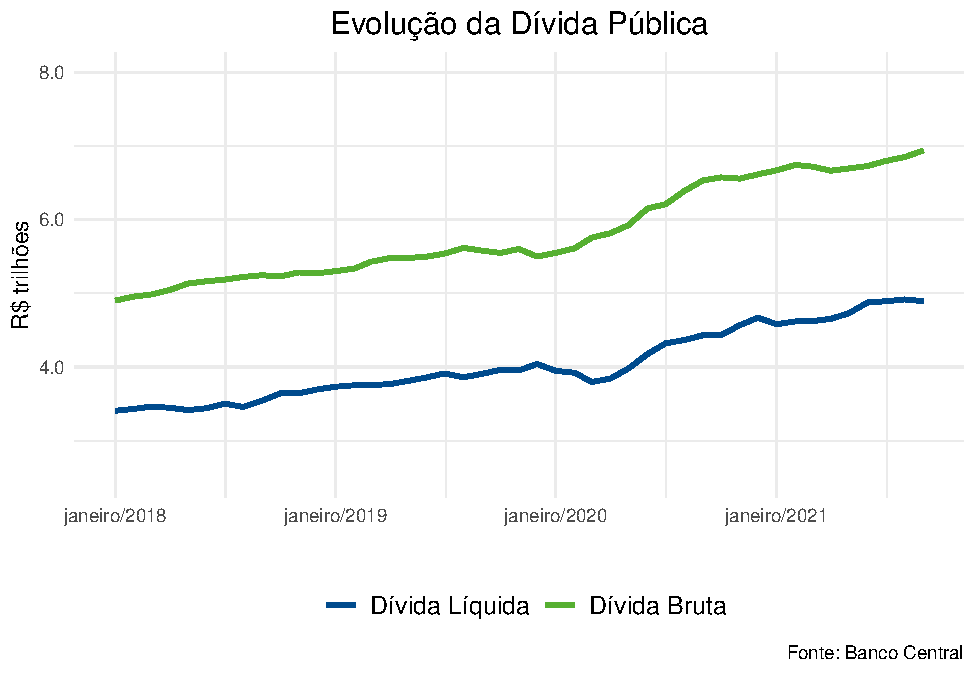
\includegraphics{politica-fiscal_files/figure-latex/Divida Liquida e Bruta-1.pdf}

Por fim, os principais indicadores que explicam a relação dívida/PIB são
os juros nominais, inflação, resultado primário e crescimento econômico.
Nesse sentido, a alta da taxa Selic para conter a expectativa de alta da
inflação pode explicar o crescimento da relação dívida/PIB. Por outro
lado, o ajuste nas contas públicas provocado pela redução das despesas
em 2021 é um fator importante para conter este avanço.

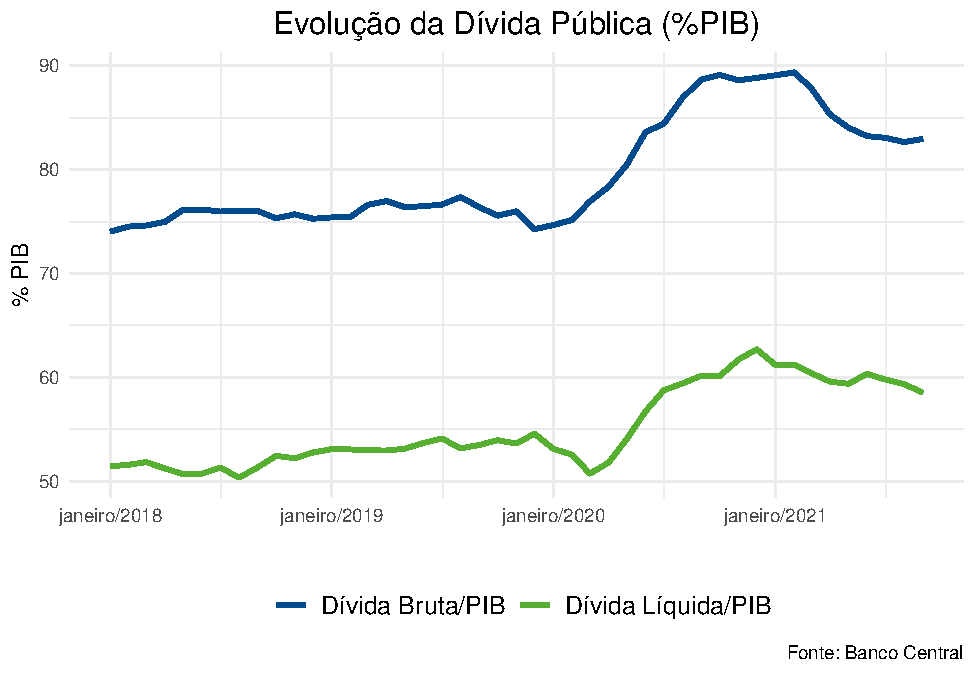
\includegraphics{politica-fiscal_files/figure-latex/Divida PIB-1.pdf}


\end{document}
